\documentclass[10pt,french]{book}

\input preambule_2013
\pagestyle{empty}

\usepackage{geometry} % package offrant une autre méthode pour redéfinir les marges
\geometry{a4paper, top=0.5cm,bottom=1cm,left=1cm,right=1cm}

\begin{document}

\begin{landscape}

\begin{multicols}{2}
On note la répartition des salariés d'une entreprise suivant le salaire mensuel. Le salaire étant un caractère continu, on peut utiliser un regroupement par classe :

\begin{center}
    \renewcommand\arraystretch{3}
        \begin{tabular}{|>\centering m{2cm}|c*{4}{|m{1.5cm}}|}
            \hline
                Tranches de salaires & Effectifs & Centre\par de classe & Fréquence fraction & Fréquence en $\%$ & FCC \\
            \hline
                $\intervallefo{0}{250}$ & $10$ & &&& \\
            \hline
                $\intervallefo{250}{500}$ & $15$ &&&& \\
            \hline
                $\intervallefo{500}{750}$ & $45$ & &&&\\
            \hline
                $\intervallefo{750}{\np{1000}}$ & $110$ &&&& \\
            \hline
                $\intervallefo{\np{1000}}{\np{1250}}$ & $255$ &&&&\\
            \hline
                $\intervallefo{\np{1250}}{\np{1500}}$ & $150$ &&&&\\
            \hline
                $\intervallefo{\np{1500}}{\np{1750}}$ & $60$ & &&&\\
            \hline
                $\intervallefo{\np{1750}}{\np{2000}}$ & $35$ & &&&\\
            \hline
                Total & & &&& \\
            \hline
        \end{tabular}
    \renewcommand\arraystretch{1}
    \end{center}

\columnbreak

\begin{center}
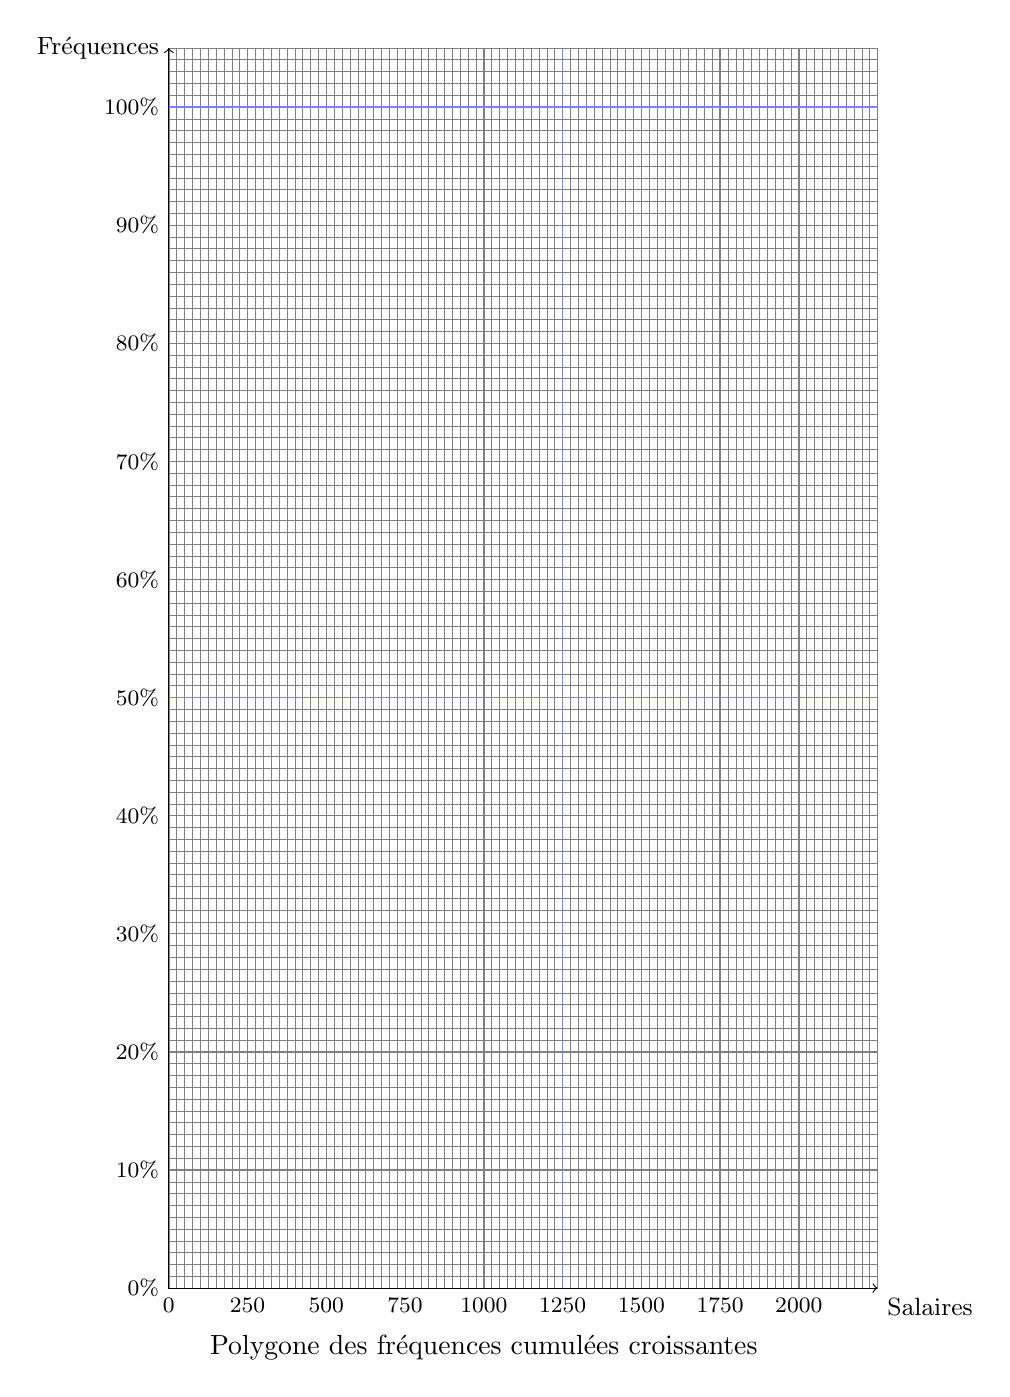
\begin{tikzpicture}[yscale=0.15]
	% Dimensions du repere
	\def\xmin{0} \def\xmax{9} \def\ymin{0} \def\ymax{105}
	% Grilles
	\draw [xstep=0.1,ystep=1,gray,very thin]  (\xmin,\ymin) grid (\xmax,\ymax);
	\draw [xstep=1,ystep=10,gray,thin] (\xmin,\ymin) grid (\xmax,\ymax);
	\draw [xstep=5,ystep=50,thin,color=blue!50]  (\xmin,\ymin) grid (\xmax,\ymax);
    \draw (4,-5) node {Polygone des fréquences cumulées croissantes};
    \draw[<->] (0,105) node[left] {\small Fréquences} -- (0,0) -- (9,0) node[below right] {\small Salaires};
    \foreach \x in {0,250,...,2000} \draw ({\x / 250},0) node[below] {\footnotesize $\x$};
    \foreach \x in {0,10,...,100} \draw (0,\x) node[left] {\footnotesize $\x\%$};
\end{tikzpicture}
\end{center}

\end{multicols}


\end{landscape}

\end{document} 